
% --------------------------------------------------------------
% This is all preamble stuff that you don't have to worry about.
% Head down to where it says "Start here"
% --------------------------------------------------------------

\documentclass[11pt]{article}

\usepackage{bera}
%\renewcommand{\familydefault}{\rmfamily}

\usepackage{graphicx,url}
\usepackage{proof}
\usepackage{framed}
\usepackage{etaremune}
\usepackage{graphics}
\usepackage[margin=0.5in]{geometry}
\usepackage{amsmath,amsthm,amssymb,amsfonts}
\usepackage{paralist}
\thispagestyle{empty}

% 1. To get version suitable for students to populate,
%    remove the contents of the \ignoreSoln{..body..}
%
% 2. To get a version suitable for generating PDF 
%    without solutions, remove the #1 below
%
% 3. To generate solutions, keep the #1 below
%
% 4. Assigned grader fills \ignoreSoln{..body..}
%    and also provides his/her feedback to student
%    and policy followed for point deduction
%    So design policy before grading begins.

\newcommand{\ignoreSoln}[1]{#1}   
%\newcommand{\ignoreModel}[1]{#1} 


\newcommand{\bigset}[2]{\big\{\;#1\;:\;#2\;\big\}}
\newcommand{\N}{\mathbb{N}}
\newcommand{\Z}{\mathbb{Z}}
\newcommand{\R}{\mathbb{R}}
\newcommand{\Np}{\mathbb{N^{+}}}

\newenvironment{theorem}[2][Theorem]{\begin{trivlist}
\item[\hskip \labelsep {\bfseries #1}\hskip \labelsep {\bfseries #2.}]}{\end{trivlist}}
\newenvironment{lemma}[2][Lemma]{\begin{trivlist}
\item[\hskip \labelsep {\bfseries #1}\hskip \labelsep {\bfseries #2.}]}{\end{trivlist}}
\newenvironment{exercise}[2][Exercise]{\begin{trivlist}
\item[\hskip \labelsep {\bfseries #1}\hskip \labelsep {\bfseries #2.}]}{\end{trivlist}}
\newenvironment{reflection}[2][Reflection]{\begin{trivlist}
\item[\hskip \labelsep {\bfseries #1}\hskip \labelsep {\bfseries #2.}]}{\end{trivlist}}
\newenvironment{proposition}[2][Proposition]{\begin{trivlist}
\item[\hskip \labelsep {\bfseries #1}\hskip \labelsep {\bfseries #2.}]}{\end{trivlist}}
\newenvironment{corollary}[2][Corollary]{\begin{trivlist}
\item[\hskip \labelsep {\bfseries #1}\hskip \labelsep {\bfseries #2.}]}{\end{trivlist}}

\DeclareMathSizes{14}{14}{14}{14}

\begin{document}

% --------------------------------------------------------------
%                         Start here
% --------------------------------------------------------------

%\renewcommand{\qedsymbol}{\filledbox}


\begin{center}
\begin{large}
  CS 6110, Spring 2022, Assignment 2  \\
  Given 1/25/22 -- Due 2/1/22 by 11:59 pm via your Github 
  \ \\
%  \ \\  
    {  {\Large\bf NAME: Tripti Agarwal} \hfill {\Large\bf UNID: u1319433 }\hspace{4cm} }
          \ \\
\end{large}

\end{center}



\begin{enumerate}
  
%- 1 ----------------------------------------------------------------
\item 
\textbf{Justice and Compassion}\newlength{\minpagw}
\settowidth{\minpagw}{\hspace{40em}}
\begin{figure}[!h]
\begin{minipage}{\minpagw}
  \fbox{%
    \parbox{1.35\linewidth}{%
    We start the x at 0 or 1. Then we set the init state to true. This means that the init state is set non-deterministically.
    \begin{itemize}
        \item \textbf{p1.pml} 
        We now want to flip the next states of x. The LTL formula says eventually x implies henceforth x. There is a point at which x is true, but this not imply that x is always from from that point. Hence this gives an error shown:\\
         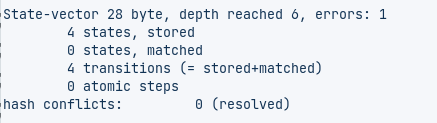
\includegraphics[width=2.7in]{p1.png}
        \item \textbf{p2.pml}
        Here the LTL formula is for henceforth x implies eventually x. This means at some point i, x is true and remains true. This does imply that x is eventually true at point i. Hence we end up getting no error.\\
        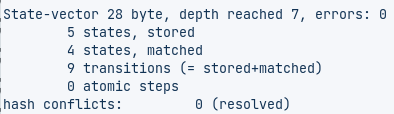
\includegraphics[width=2.7in]{p2.png}
        \item \textbf{p3.pml}
         \textbf{Justice:} (<>[]x -> []<>y)
i.e. eventually-henceforth x then infinitely-often y.
\textbf{Compassion:} ([]<>x -> []<>y)
i.e. infinitely-often x then infinitely-often y  In p3, it is \textbf{compassion implies justice}. As compassion is strong fairness and it make sense that if we infinitely often perform an action then infinitely often other action will happen. This does definitely imply that at some point an action is true then we are performing infinitely often other action. 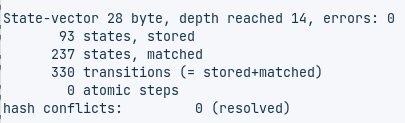
\includegraphics[width=2.7in]{p3.png}
        
        \item \textbf{p4.pml}
        In p4, the LTL formula is for \textbf{justice imply compassion}. As we can see justice means weak fairness, and it is eventually henceforth an action then infinitely often other action will happen. This does not imply, that if we infinitely often keep doing an action then infinitely often other action will also happen. Hence we end up getting an error.\\ 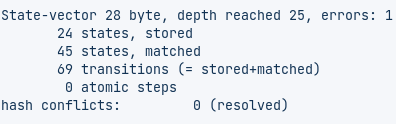
\includegraphics[width=2.7in]{p4.png}
        \item \textbf{Justice imply compassion?}
        From example p4.pml it is clear that justice does not imply compassion. \textbf{Compassion imply justice?}
        From example p3.pml it is clear that compassion imply justice.
        \item \textbf{Pnueli's paper's title true?} 
        \item \begin{enumerate}
         \item The solicitor is walking around in round robin fashion and knocking at each door. Since the home-owners are found to be infinitely-often opening and closing, therefore this is \textbf{strong fairness} or \textbf{compassionate}. Here $\tau$ (solicitor knocking at the door) is infinitely often enabled and the home owners are bound to open and then close the door infinitely many times.
         \item Since the solicitor walks at one door and keep on pressing the bell till it melts, i.e this transition is continuously enabled and then the home owner infinitely-often opens the door, therefore in this case the home owners have \textbf{weak fairness} or \textbf{justice}. 
         \item If the solicitor is a network packet and the home owner doors are ports, then in first case (a), the network packet reaches every port and ask whether the port is open and repeats this for all the ports and hence this is called compassion. Whereas in case (b), the packet comes at one port and waits there till the time the port is open and this is called justice.
         
     \end{enumerate}
    \end{itemize}
      
    }%
  }%
\end{minipage}
\end{figure}
\clearpage
  

%- 2 ----------------------------------------------------------------
\newpage
\item \textbf{LTL for sa and sb kripke structure}
\begin{figure}[!h]
\begin{minipage}{\minpagw}
  \fbox{%
    \parbox{1.3\linewidth}{%
      \begin{enumerate}
          \item After changing the never automata with the corresponding LTL formula we can see that Sb gives no erro with both the LTLs. This is because Sb is true for both and Sa works only with second LTL. Proofs for the above are provided in the snipet shown below.
           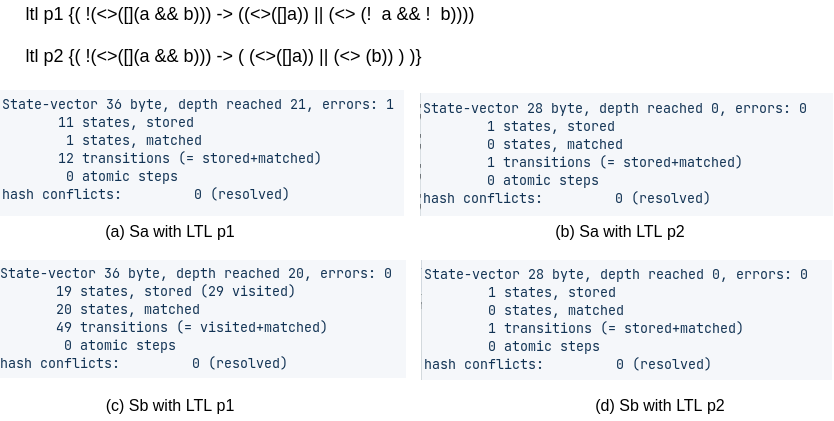
\includegraphics[width=5.0in]{ltl.png}
           \item
        \begin{enumerate}
            \item \textbf{Does sa implies sb?} No sa do not imply sb. This can be observed from the error traces obtained from LTL formulas. We can see the LTL formula p1 can result in an error for sa and not for sb. Similiary for p2 both sa and sb satisfies. This means, the kripke structure of sa cannot give full information of sb. Hence LTL of sa do no imply sb.
       \item \textbf{Does LTL of sb implies sa?} Yes, sb implies sa. This can be observed from LTL p1 and p2. We see p2 satisfies both sa and sb, but p1 only satisfies sb. This means the the LTL formula for sb can imply LTL formula for sa.
        \end{enumerate} \end{enumerate}
    }%
  }%
\end{minipage}
\end{figure}
\clearpage

%- 3 ----------------------------------------------------------------

\item  \textbf{Bubble sort}
\begin{figure}[!h]
\begin{minipage}{\minpagw}
  \fbox{%
    \parbox{1.2 \linewidth}{%
      \begin{itemize}
          \item \textbf{Fixed broken bubble sort} The bubble sort code was broken at line 31 and 42 of the code. The value of t was assigned to a[1] whereas it should be assigned as 1. Also, the code is further enhanced, as the bubble sort is sorting the maximum value first and putting it at the end. The code provided in the github repo, is an optimized version where the loop is decreased by 1 every time the maximum element is pushed to end.
          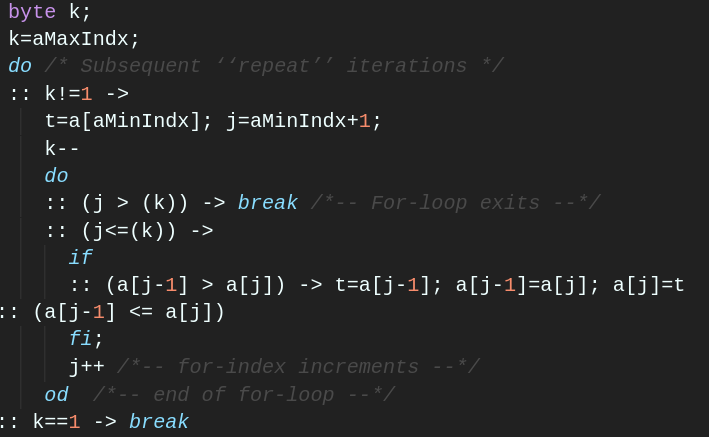
\includegraphics[width=3.0in]{bubble.png}
          \item \textbf{Evidence that the code has been checked exhaustively}
          \begin{itemize}
              \item \textit{Ran the code for depth 10, no error obtained}\\
              \centering
                    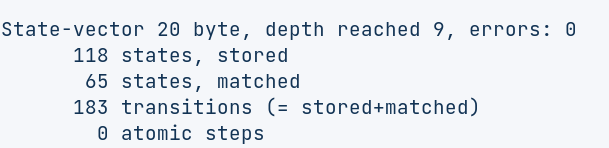
\includegraphics[width=3.0in]{bubble_10.png}
              \item \textit{Ran the code for depth 20, no error obtained}
              
                    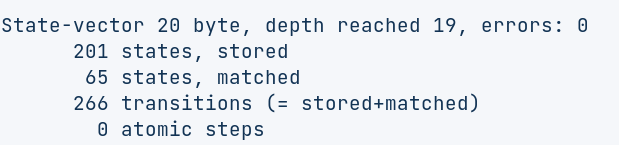
\includegraphics[width=3.0in]{bubble_20.png}
              \item \textit{Ran the code for depth 30, no error obtained} \\The maximum depth was till 27 and still we did not get any error. Hence we have ran the code exhaustively to check that the code is now correct.
              
                    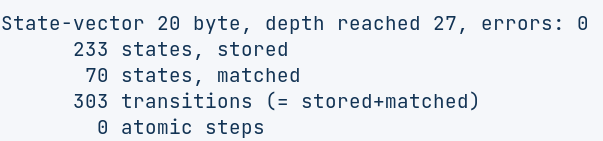
\includegraphics[width=3.0in]{bubble_30.png}
          \end{itemize}
          \item \textbf{Increasing the size of array}
         \\ 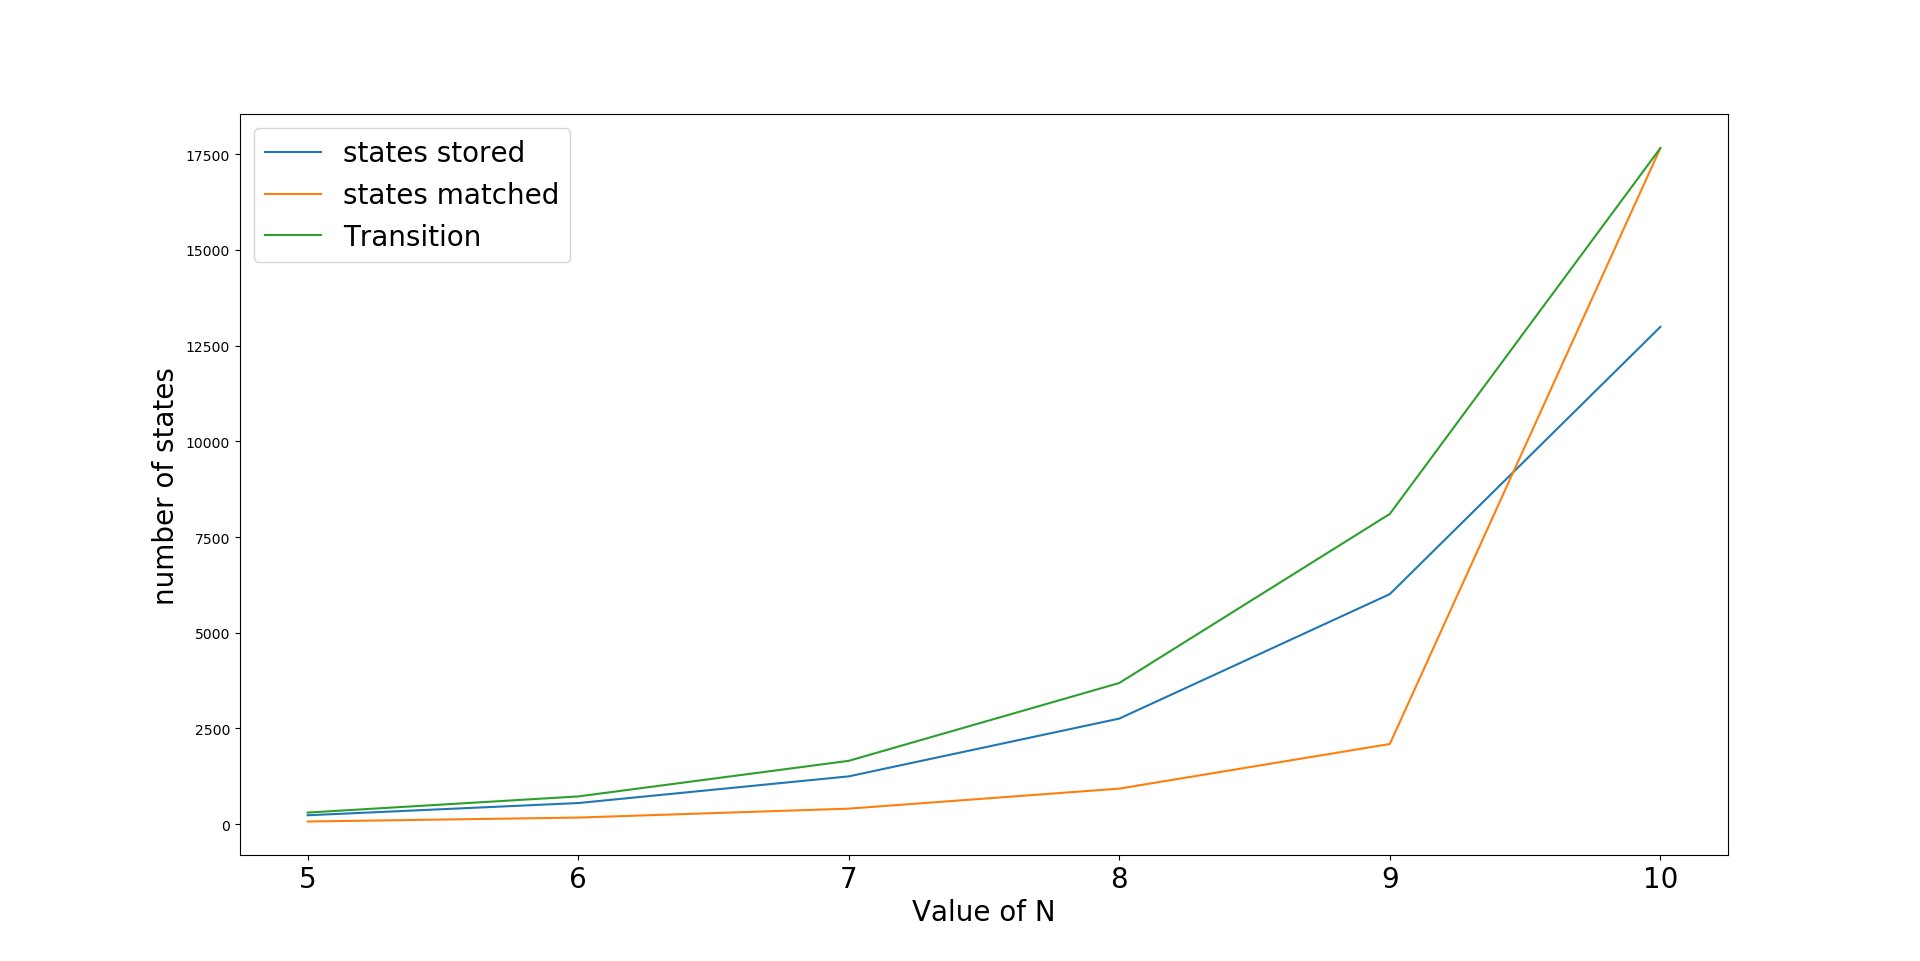
\includegraphics[width=4.2in]{bubble_plot.png}
      \end{itemize}
    }%
  }%
\end{minipage}
\end{figure}

\clearpage

%- 4 ----------------------------------------------------------------
\item \textbf{Dinning Philosopher's code}
  
\begin{figure}[!h]
\begin{minipage}{\minpagw}
  \fbox{%
    \parbox{\linewidth}{%
     
          The code is ran exhaustively to obtain following traces. The code works fine without any error.\\
          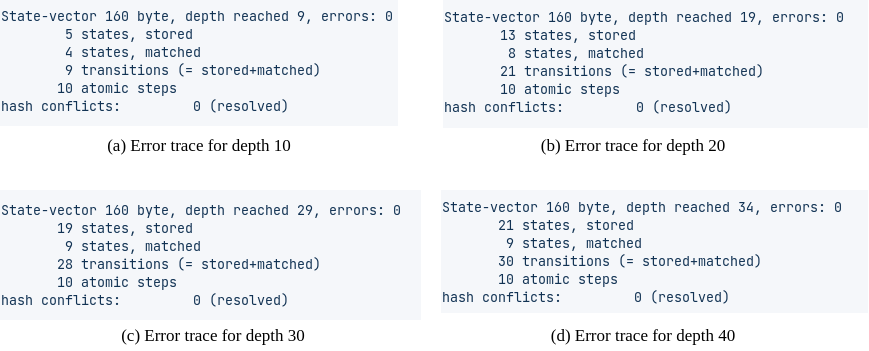
\includegraphics[width=5.0in]{Phill.png}
          
    
    }%
}
\end{minipage}
\end{figure}  
\clearpage

%- 5 ----------------------------------------------------------------
\item \textbf{DT.pml}
  
\begin{figure}[!h]
\begin{minipage}{\minpagw}
  \fbox{%
    \parbox{1.3\linewidth}{%
      The code with the changes are available on Github. Here is the change in the code for the work assignment from any node to upstream root node. The code did not had the case when we pick the root node. The code is also changed for the random initialization given in the question.
      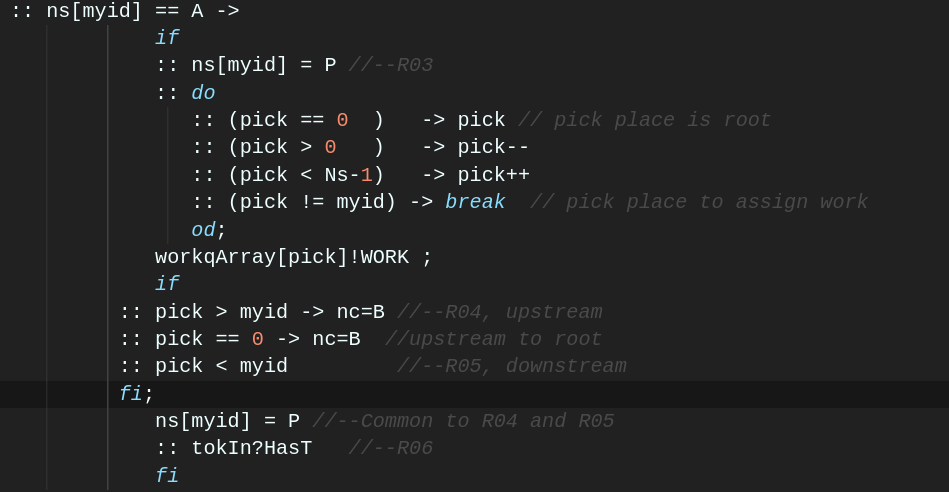
\includegraphics[width=5.0in]{DT_root.png}\\
      The code is run exhaustively for different depth. For depth of 50000, we get 43215 with no error as shown in the figure below.\\
      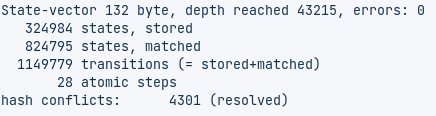
\includegraphics[width=5.0in]{DT_output.png}\\
      Plot for different values of N for states stored, matched and no of transition states.\\
      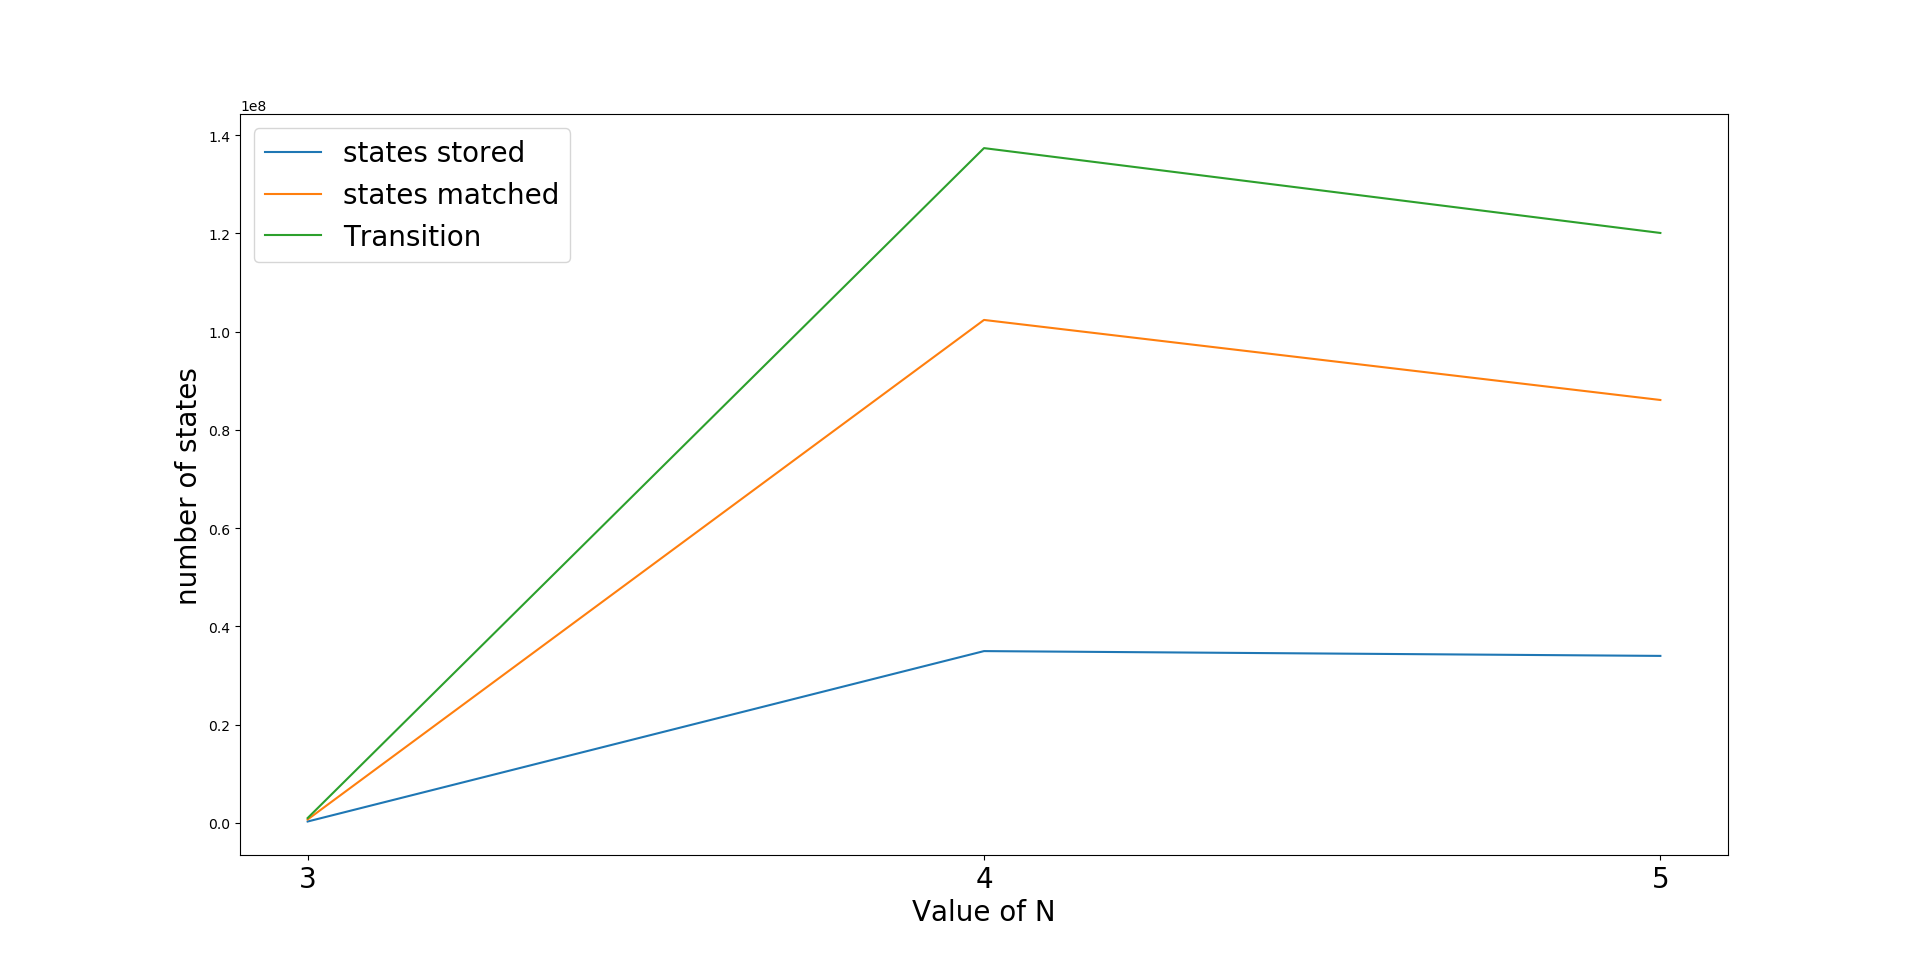
\includegraphics[width=6.0in]{DT_plot.png}
    }%
  }%
\end{minipage}
\end{figure}
% --------------------------------------------------------------
\end{enumerate}

\end{document}